\documentclass[11pt]{article}

\marginparwidth 0.0in 
\oddsidemargin 0.05in 
\evensidemargin 0.05in 
\marginparsep 0.05in
\topmargin 0.05in 
\textwidth 6in \textheight 8 in

\usepackage{amsmath}
\usepackage{upgreek}
\usepackage{graphicx}
\usepackage{listings}

\date{15 December 2017}
\begin{document}
\author{Pedro Tavares \\ \texttt{up201708899@fe.up.pt} \and Raquel Dias \\ \texttt{up201700419@fe.up.pt} }
\title{Model-Based Testing Assignment}

\maketitle

\textbf{Note}: You should have \texttt{Java 8+} and \texttt{Maven 3.5.0+} installed on your local machine. \\

\textbf{Before we start}: Make sure that you are at the root assignment folder.
In order to open MISTA, execute the following command: \texttt{java -jar MISTA1.0/MISTA.jar}. Go to \texttt{File->Open}, navigate to \texttt{assignment->src->test->java->tvvs}, and select the \texttt{VendingMachine.xmid} file. Then, go to \texttt{Test->Options} and uncheck the \textit{Add object reference to accessors} option. In order to edit the assignment source code and execute the generated tests, open/import the \texttt{assignment} folder with you favorite IDE.\\

Given the Petri Net defined on Figure \ref{fig:petri-net}:

\begin{figure}[!htb]
    \centering
    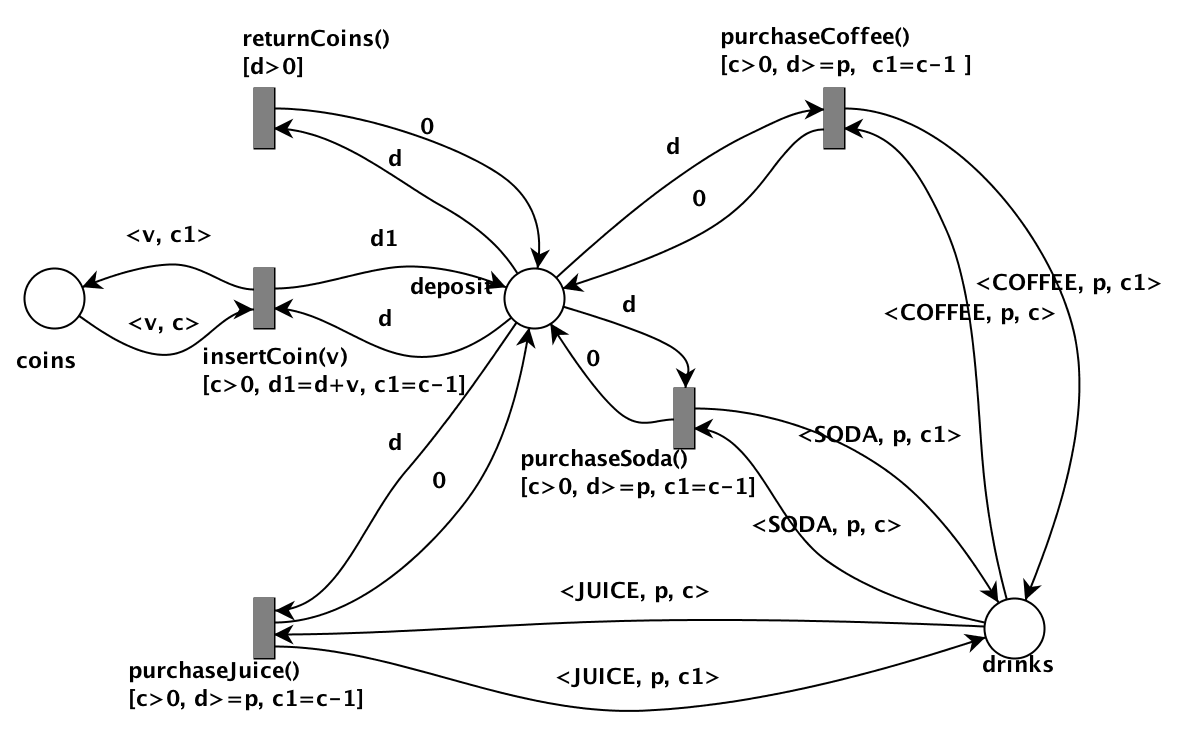
\includegraphics[scale=0.65]{petri-net.png}
    \caption{Petri Net that represents a vending machine system.}
    \label{fig:petri-net}
\end{figure}

\begin{enumerate}

\item Implement the following methods on \texttt{VendindMachine} class:

\texttt{void insertCoin(Coin coin);} \\ 
\texttt{void returnCoins();} \\
\texttt{void purchase(String drink);} \\

\item With MISTA opened, go to \texttt{MIM -> Methods} and map the Model-Level Events to the actual implementation code:

\begin{table}[!htb]
\centering
\begin{tabular}{|l|c|}
\hline
\textbf{Model-Level Event} & \textbf{Implementation Code}\\
\hline
\texttt{insertCoin(1)} & ?\\
\texttt{insertCoin(5)} & ?\\
\texttt{insertCoin(10)} & ?\\
\texttt{insertCoin(25)} & ?\\
\texttt{insertCoin(100)} & ?\\
\texttt{returnCoins()} & ?\\
\texttt{purchaseCoffee()} & ?\\
\texttt{purchaseJuice()} & ?\\
\texttt{purchaseSoda()} & ?\\
\hline
\end{tabular}
\caption{Empty mapping from Model-Level Event to Implementation Code}
\end{table}

\item With the setup defined on Listing \ref{lst:petri-net-setup-1}, generate test cases based on the Reachability Tree coverage criteria (Select \texttt{Reachability Tree}, \texttt{Java}, and \texttt{JUnit}. Finally, go to \texttt{Test->Generate Test Code}). A file should be created inside the test folder. Run the generated tests with JUnit. \textbf{Note[1]}: before running the test generation, try to guess the number of tests that will cover the criteria. Compare the number and share your thoughts. \textbf{Note[2]}: The tests should pass. If they're failing, look for inconsistencies in both model and implementation. If you find any, fix it and re-generate the tests. Remember, a wrongly designed model can lead to unreliable test results.

\begin{lstlisting}[label={lst:petri-net-setup-1},language=Java,basicstyle=\ttfamily,keywordstyle=\color{red},caption={This setup allow a maximum of four coins per test case, one per coin type (5, 10, 25, and 100). Deposit starts at 0. Each drink has it own price.}, captionpos=b]
INIT coins(5,1), coins(10,1), coins(25,1),
coins(100,1), deposit(0), drinks(COFFEE,35,1),
drinks(JUICE,110,1), drinks(SODA,105,1)
\end{lstlisting}

\item Change the setup values in order to accept more coins on each test scenario. Again, try to guess the number of test cases, obverse the test generation, execute the tests, and share your thoughts.

\item Repeat the process for other coverage criteria: Transition, State and Depth coverage.

\end{enumerate}
\end{document}
